\documentclass[12pt,]{article}
\usepackage{lmodern}
\usepackage{amssymb,amsmath}
\usepackage{ifxetex,ifluatex}
\usepackage{fixltx2e} % provides \textsubscript
\ifnum 0\ifxetex 1\fi\ifluatex 1\fi=0 % if pdftex
  \usepackage[T1]{fontenc}
  \usepackage[utf8]{inputenc}
\else % if luatex or xelatex
  \ifxetex
    \usepackage{mathspec}
  \else
    \usepackage{fontspec}
  \fi
  \defaultfontfeatures{Ligatures=TeX,Scale=MatchLowercase}
\fi
% use upquote if available, for straight quotes in verbatim environments
\IfFileExists{upquote.sty}{\usepackage{upquote}}{}
% use microtype if available
\IfFileExists{microtype.sty}{%
\usepackage{microtype}
\UseMicrotypeSet[protrusion]{basicmath} % disable protrusion for tt fonts
}{}
\usepackage[margin=0.50in]{geometry}
\usepackage{hyperref}
\hypersetup{unicode=true,
            pdftitle={Analysis of integration site distributions and clonal abundances for gene therapy correction of cystinosis},
            pdfauthor={John K. Everett, Ph.D.~and Frederic Bushman, Ph.D.},
            pdfborder={0 0 0},
            breaklinks=true}
\urlstyle{same}  % don't use monospace font for urls
\usepackage{graphicx,grffile}
\makeatletter
\def\maxwidth{\ifdim\Gin@nat@width>\linewidth\linewidth\else\Gin@nat@width\fi}
\def\maxheight{\ifdim\Gin@nat@height>\textheight\textheight\else\Gin@nat@height\fi}
\makeatother
% Scale images if necessary, so that they will not overflow the page
% margins by default, and it is still possible to overwrite the defaults
% using explicit options in \includegraphics[width, height, ...]{}
\setkeys{Gin}{width=\maxwidth,height=\maxheight,keepaspectratio}
\IfFileExists{parskip.sty}{%
\usepackage{parskip}
}{% else
\setlength{\parindent}{0pt}
\setlength{\parskip}{6pt plus 2pt minus 1pt}
}
\setlength{\emergencystretch}{3em}  % prevent overfull lines
\providecommand{\tightlist}{%
  \setlength{\itemsep}{0pt}\setlength{\parskip}{0pt}}
\setcounter{secnumdepth}{0}

%%% Use protect on footnotes to avoid problems with footnotes in titles
\let\rmarkdownfootnote\footnote%
\def\footnote{\protect\rmarkdownfootnote}

%%% Change title format to be more compact
\usepackage{titling}

% Create subtitle command for use in maketitle
\newcommand{\subtitle}[1]{
  \posttitle{
    \begin{center}\large#1\end{center}
    }
}

\setlength{\droptitle}{-2em}
  \title{Analysis of integration site distributions and clonal abundances for
gene therapy correction of cystinosis}
  \pretitle{\vspace{\droptitle}\centering\huge}
  \posttitle{\par}
  \author{John K. Everett, Ph.D.~and Frederic Bushman, Ph.D.}
  \preauthor{\centering\large\emph}
  \postauthor{\par}
  \predate{\centering\large\emph}
  \postdate{\par}
  \date{August 2018}

\usepackage{booktabs}
\usepackage{longtable}
\usepackage{array}
\usepackage{multirow}
\usepackage[table]{xcolor}
\usepackage{wrapfig}
\usepackage{float}
\usepackage{colortbl}
\usepackage{pdflscape}
\usepackage{tabu}
\usepackage{threeparttable}
\usepackage[normalem]{ulem}

\usepackage{caption}

\begin{document}
\maketitle

{
\setcounter{tocdepth}{2}
\tableofcontents
}
\captionsetup[table]{labelformat=empty}

\newpage

\section{Summary of results}\label{summary-of-results}

The goal of this analysis is to investigate the integration profile of a
gene therapy vector for the correction of cystinosis in mouse subjects
and assess potential clonal expansions. The list of mouse oncogenes was
compiled from the retroviral tagged cancer gene database
(RTCGD)\textsuperscript{1} using an inclusion threshold of three or more
incidents where the mouse oncogene list comprises 2.01\% of all mouse
genes. The frequency of integration near oncogenes was generally less
than that of mice in a previously published \(\beta\)-thalassemia mouse
trial from which no adverse events have been reported
\textsuperscript{2}. The code base for this analysis is available online
(\href{https://github.com/everettJK/project.geneTherapy.ucsdMouseCystinosis}{link}).

\vspace{0.1cm}

\section{Mouse samples studied}\label{mouse-samples-studied}

Integration sites were detected in 16 samples from mouse subjects
(Tables 1 \& S1).

\vspace{0.1cm}

\begin{table}[!h]

\caption{\label{tab:unnamed-chunk-2}Table 1. Overview of data collection.}
\centering
\begin{tabular}[t]{ccccc}
\toprule
Organism & Number of samples & Number of reads & Number of inferred cells & Number of integration sites\\
\midrule
mouse & 16 & 9,464,092 & 29,630 & 2,346\\
\bottomrule
\end{tabular}
\end{table}

\vspace{0.5cm}

\section{Subject reports}\label{subject-reports}

Subject specific reports for all subjects are available via a protected
web archive
(\href{http://www.bushmanlab.org/data/export/cherqui}{link}).\\
user: cherqui\\
pass: geneTherapy@!\#

\vspace{0.5cm}

\section{UCSC browser exploration}\label{ucsc-browser-exploration}

UCSC browser sessions pre-loaded with the integration sites identified
in this analysis are available via this\\
(\href{http://genome.ucsc.edu/cgi-bin/hgTracks?org=mouse\&db=mm9\&hgt.customText=http://microb120.med.upenn.edu/UCSC/cherqui/UCSC_CYS_mouse.group2.ucsc}{link}).
Integration sites are shown as blue (positive orientation integration)
and red (reverse orientation integration) tick marks. For each
integration site, a second track provides the maximum clonal abundance.
Entering gene names into the search bar will direct the browser to
specific genes.

\newpage

\section{Description of analysis
techniques}\label{description-of-analysis-techniques}

We investigate effects of integration on cell growth using the following
criteria: Integration Frequency is the frequency at which unique
integration sites are observed in or near a given gene. Clonal Abundance
is determined by quantifying the number of sites of linker ligation
associated with each unique integration site. This samples the number of
DNA chains at the start of the experiment allowing clonal expansion to
be quantified\textsuperscript{4}.

Relative clonal Abundance is determined per sample and is the percentage
of identified cells attributed to a given clone. Integration sites and
the clones harboring them are sampled from a larger population. It would
be rare for all integration sites in a sample to be represented in the
sequence data.

For this analysis, four technical replicates of each delivered sample
were prepared, sequenced and analyzed with the INSPIIRED integration
site analysis pipeline (v1.2)\textsuperscript{4}.

\newpage

\section{Comparisons to previous
trials}\label{comparisons-to-previous-trials}

\subsection{Integration events near oncogenes in mouse
subjects}\label{integration-events-near-oncogenes-in-mouse-subjects}

\vspace{0.1cm}

In order to determine if the experimental vector has a higher propensity
of integrating near suspected oncogene in mice than previously employed
vectors, the frequency of integration near oncogenes was compared to a
previously published mouse trial\textsuperscript{2} which used a
comparable lentiviral vector to correct \(\beta\)-thalassemia. The
frequency of integration events near oncogenes was generally less than
the mean frequency of integration events near oncogenes in the published
trial (Figure 1 {[}CYS: gray, \(\beta\)-thalassemia trial: blue{]}).

\vspace{1.0cm}

\emph{Figure 1. Comparison of frequencies of integration events near
oncogenes.}

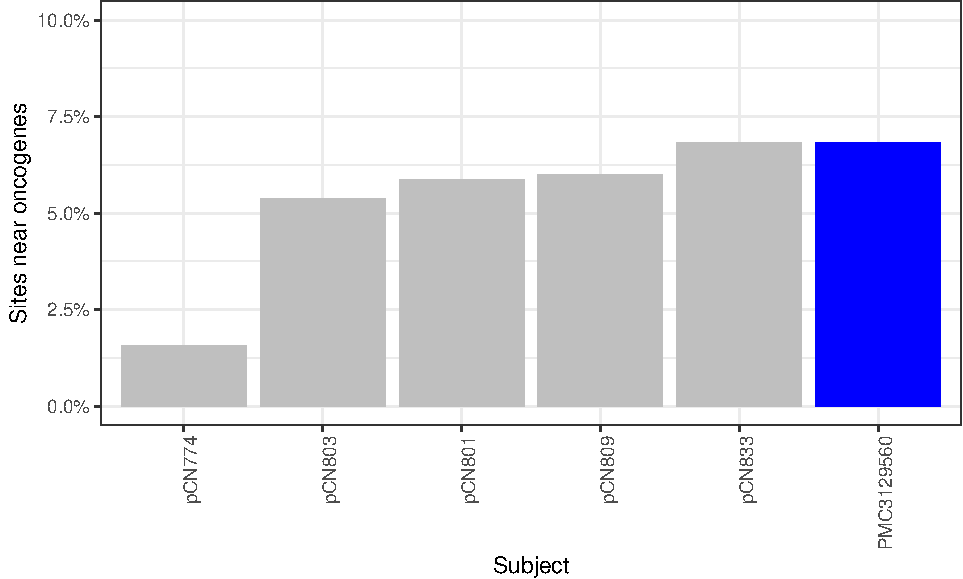
\includegraphics{project.group2_files/figure-latex/fig1-1.pdf}

\newpage

\section{Mapping of integration site
positions}\label{mapping-of-integration-site-positions}

Heat map of identified integration positions is shown below in Figure 2.

\emph{Figure 2}

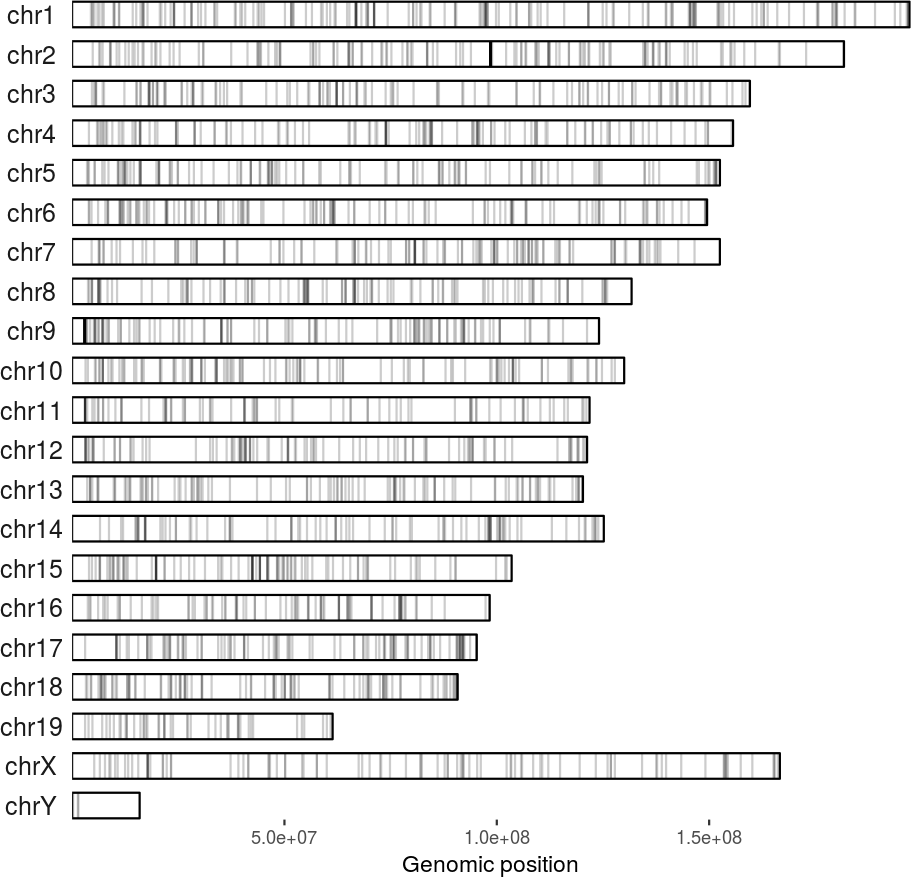
\includegraphics{project.group2_files/figure-latex/fig2-1.png}

\newpage

\section{Relative abundances of mouse subject
samples}\label{relative-abundances-of-mouse-subject-samples}

The sample relative abundance plots below (Figure 3) show the most
abundant 25 clones in each sample as colored bars while less abundant
clones were relegated to a single low abundance bar shown in gray.

\emph{Figure 3.}

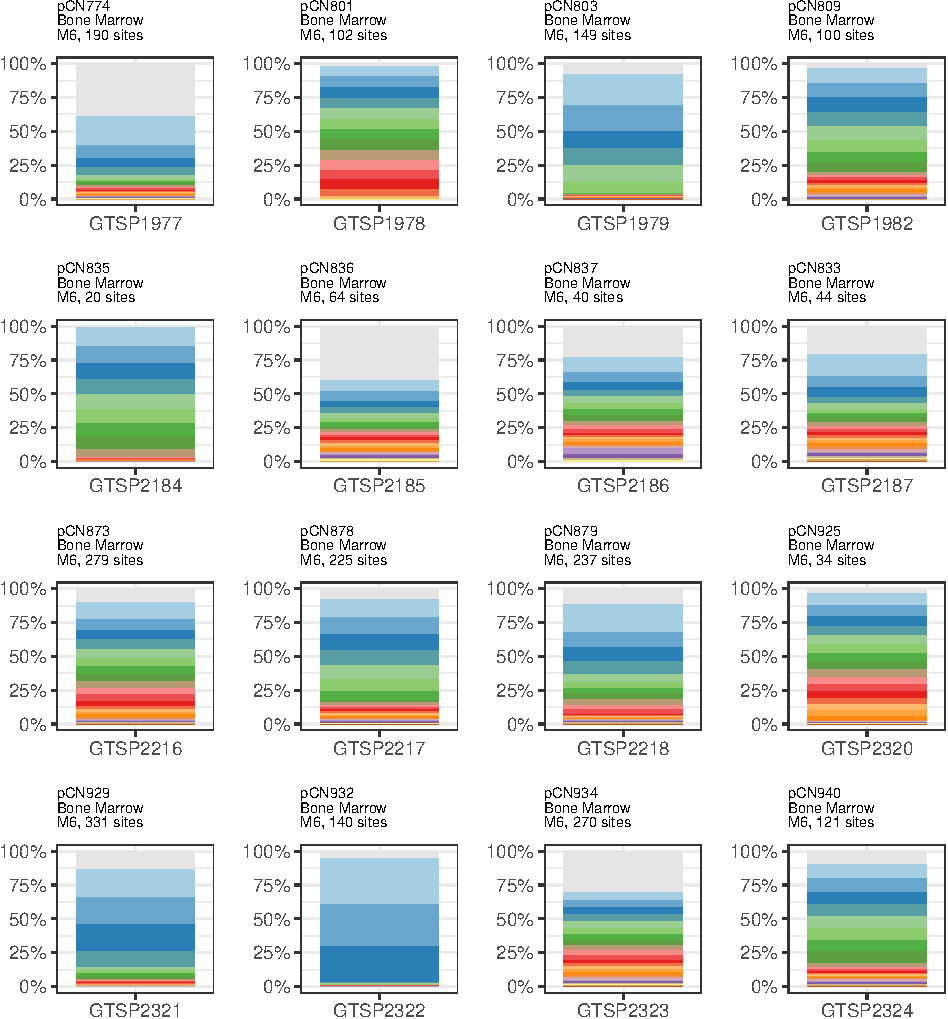
\includegraphics{project.group2_files/figure-latex/fig3-1.pdf}

\newpage

\section{Expanded clones}\label{expanded-clones}

Table 2 below lists clones with relative clonal abundances \(\geq\)
20\%. The estimated number of cells harboring each integration
(Abundance) is shown for context.

\emph{Table 2.}

\begin{table}[H]
\centering\rowcolors{2}{gray!6}{white}

\resizebox{\linewidth}{!}{\begin{tabular}{llllllrl}
\hiderowcolors
\toprule
Subject & Organism & Time point & Cell type & Position & Relative abundance & Abundance & Nearest gene\\
\midrule
\showrowcolors
pCN774 & mouse & M6 & Bone Marrow & chr1-21011655 & 22.15\% & 107 & Tram2\\
pCN929 & mouse & M6 & Bone Marrow & chr12-38193729 & 22.61\% & 548 & Agmo\\
pCN932 & mouse & M6 & Bone Marrow & chr12+80277915 & 35.25\% & 553 & Rdh11\\
pCN932 & mouse & M6 & Bone Marrow & chr8-66234933 & 25.56\% & 401 & Sgo2b\\
pCN932 & mouse & M6 & Bone Marrow & chr8+9405148 & 25.30\% & 397 & Fam155a\\
\bottomrule
\end{tabular}}
\rowcolors{2}{white}{white}
\end{table}

\newpage

\textbf{Analyst}


\includegraphics[width=4.04in]{./data/Everett_signature}

John K. Everett, Ph.D.

\vspace{0.5cm}

\textbf{Laboratory director}


\includegraphics[width=5.99in]{./data/Bushman_signature}

Frederic D. Bushman, Ph.D.

\vspace{2.0cm}

\section{References}\label{references}

\begin{enumerate}
\def\labelenumi{\arabic{enumi}.}
\tightlist
\item
  RTCGD: retroviral tagged cancer gene database. Akagi K, Suzuki T,
  Stephens RM, Jenkins NA, Copeland NG. Nucleic Acids Res. 2004 Jan
  1;32(Database issue):D523-7.
\end{enumerate}

\vspace{0.1cm}

\begin{enumerate}
\def\labelenumi{\arabic{enumi}.}
\setcounter{enumi}{1}
\tightlist
\item
  Distribution of Lentiviral Vector Integration Sites in Mice Following
  Therapeutic Gene Transfer to Treat \(\beta\)-thalassemia. Ronen K,
  Negre O, Roth S, Colomb C, Malani N, Denaro M, Brady T, Fusil F,
  Gillet-Legrand B, Hehir K, Beuzard Y, Leboulch P, Down JD, Payen E,
  Bushman FD. Mol Ther. 2011 Jul;19(7):1273-86.
\end{enumerate}

\vspace{0.1cm}

\begin{enumerate}
\def\labelenumi{\arabic{enumi}.}
\setcounter{enumi}{2}
\tightlist
\item
  Estimating abundances of retroviral insertion sites from DNA fragment
  length data. Berry CC, Gillet NA, Melamed A, Gormley N, Bangham CR,
  Bushman FD. Bioinformatics. 2012 Mar 15;28(6):755-62.
\end{enumerate}

\vspace{0.1cm}

\begin{enumerate}
\def\labelenumi{\arabic{enumi}.}
\setcounter{enumi}{3}
\tightlist
\item
  INSPIIRED: A Pipeline for Quantitative Analysis of Sites of New DNA
  Integration in Cellular Genomes. Sherman E, Nobles C, Berry CC, Six E,
  Wu Y, Dryga A, Malani N, Male F, Reddy S, Bailey A, Bittinger K,
  Everett JK, Caccavelli L, Drake MJ, Bates P, Hacein-Bey-Abina S,
  Cavazzana M, Bushman FD. Mol Ther Methods Clin Dev. 2016 Dec
  18;4:39-49.
\end{enumerate}

\newpage

\section{Supplementary tables and
figures}\label{supplementary-tables-and-figures}

\subsection{Numbers of inferred cells and integration sites identified
in provided
samples}\label{numbers-of-inferred-cells-and-integration-sites-identified-in-provided-samples}

\emph{Table S1.}\\

\begin{table}[H]
\centering\rowcolors{2}{gray!6}{white}

\resizebox{\linewidth}{!}{\begin{tabular}{llllrlll}
\hiderowcolors
\toprule
Organism & GTSP & Subject & Cell type & VCN & Time point & Number inferred cells & Number of intSites\\
\midrule
\showrowcolors
mouse & GTSP1977 & pCN774 & Bone Marrow & 0.039 & M6 & 483 & 190\\
mouse & GTSP1978 & pCN801 & Bone Marrow & 10.490 & M6 & 3,397 & 102\\
mouse & GTSP1979 & pCN803 & Bone Marrow & 0.654 & M6 & 1,827 & 149\\
mouse & GTSP1982 & pCN809 & Bone Marrow & 0.572 & M6 & 2,765 & 100\\
mouse & GTSP2184 & pCN835 & Bone Marrow & 1.270 & M6 & 404 & 20\\
mouse & GTSP2185 & pCN836 & Bone Marrow & 2.970 & M6 & 99 & 64\\
mouse & GTSP2186 & pCN837 & Bone Marrow & 1.720 & M6 & 63 & 40\\
mouse & GTSP2187 & pCN833 & Bone Marrow & 1.070 & M6 & 93 & 44\\
mouse & GTSP2216 & pCN873 & Bone Marrow & 0.790 & M6 & 4,716 & 279\\
mouse & GTSP2217 & pCN878 & Bone Marrow & 1.260 & M6 & 3,657 & 225\\
mouse & GTSP2218 & pCN879 & Bone Marrow & 1.060 & M6 & 3,469 & 237\\
mouse & GTSP2320 & pCN925 & Bone Marrow & 0.040 & M6 & 375 & 34\\
mouse & GTSP2321 & pCN929 & Bone Marrow & 2.000 & M6 & 2,424 & 331\\
mouse & GTSP2322 & pCN932 & Bone Marrow & 1.750 & M6 & 1,569 & 140\\
mouse & GTSP2323 & pCN934 & Bone Marrow & 0.510 & M6 & 2,820 & 270\\
mouse & GTSP2324 & pCN940 & Bone Marrow & 0.140 & M6 & 1,469 & 121\\
\bottomrule
\end{tabular}}
\rowcolors{2}{white}{white}
\end{table}


\end{document}
